\documentclass[oneside,a4paper,14pt,final]{extreport}

\usepackage{essay}
%%%%%%%%%%%%%%%%%%%%%%%%%%%%%%%%%%%%%%%%%%%%%%%%%%%
%                                                 %
%              declare math operators             %
%                                                 %
%%%%%%%%%%%%%%%%%%%%%%%%%%%%%%%%%%%%%%%%%%%%%%%%%%%
% https://tex.stackexchange.com/questions/67506/newcommand-vs-declaremathoperator
% \DeclareMathOperator{\End}{End}
\DeclareMathOperator*{\argmax}{arg\,max}
\DeclareMathOperator*{\argmin}{arg\,min}
\DeclareMathOperator*{\lh}{Likelihood}
\DeclareMathOperator*{\sign}{sign}

\graphicspath{ {./graphics/} }
\addbibresource{./chapters/library.bib}

\begin{document}

\includepdf[page={1}]{./chapters/title.pdf}
%%%%%%%%%%%%%%%%%%%%%%%%%%%%%%%%%%%%%%%%%%%%%%%%%%%
\chapter*{РЕФЕРАТ}

% Использование нейронных сетей и методов машинного обучения для сентимент-анализа текстов

% Введение
%   Общее описание и актуальность задачи
%   Цель работы
%   Практическая значимость
%
% Теоретическая часть
%   Сентимент-анализ текстов
%   Виды классификации со ссылками на исследования (включая краткий обзор этих исследования)
%       По количеству классов
%       По подходам к анализу
%   Подготовка данных перед сеткой
%   Teория
%       TF-IDF, CBOW
%       Embeddings
%   Теория по ML
%   Метрики
%   Теория по RB методу

%
% Практическая часть
%   Используемые иструменты
%   Сбор данных
%   Реализация и результаты ML
%   Реализация и результаты RB
%
% Заключение
%
% Список источников
%
% Приложение
%   Toloka
%   ML & DL
%   RB

\par
Выпускная квалификационная работа содержит \pageref*{LastPage}~страниц, \totfig~рисунка,                                        \tottab~таблицу, XX использованных источника.
\bigskip

\par
КЛЮЧЕВОЕ СЛОВО 1, КЛЮЧЕВОЕ СЛОВО 2, …
\bigskip


\par
Краткое описание содержания работы.


\thispagestyle{empty} % unnumbered page

{\linespread{0.9}\tableofcontents}

\chapter*{ВВЕДЕНИЕ}
\addcontentsline{toc}{chapter}{ВВЕДЕНИЕ}


%%%%%%%%%%%%%%%%%%%%%%%%%%%%%%%%%%%%%%%%%%%%%%%%%%%
{\CenterChapterHeading\chapter*{ОСНОВНАЯ ЧАСТЬ}
\addcontentsline{toc}{chapter}{ОСНОВНАЯ ЧАСТЬ}
\newpage
}
%%%%%%%%%%%%%%%%%%%%%%%%%%%%%%%%%%%%%%%%%%%%%%%%%%%
\chapter{Теоретическая часть}

\bigskip\par
\textcolor{red}{В этой части мы подробнее раскроем теорию.}

\subsection{Обзор предметной области}

% \begin{definition}
%  Классификация текста --- использование математических моделей для определения принадлежности текста, на
основании его содержимого, к конкретному классу из определенного множества.
% \end{definition}
%
% \begin{definition}
%  Мультиклассификатор текстов --- алгоритм или обученная модель, предсказывающие принадлежность каждого
входного текста к одному или нескольким классам, множество классов определено заранее.
% \end{definition}
%
% \begin{definition}
%  Сентимент-анализ (анализ тональности) --- автоматическое выявление в текстах эмоционально окрашенной
лексики и эмоциональной оценки авторов.
% \end{definition}
%
% \begin{definition}
%  Сентимент --- совокупность чувств и взглядов, как основа для действия или суждения; общая эмоциональная
установка.
% \end{definition}

%%% 1. Semina %%%
\par
Сентимент-анализ, как направление компьютерной лингвистики, стал очень популярен последние десятилетие. С
появлением больших данных насыщенных эмоциональной составляющей возникла потребность в их обработке. Компании
начали устраивать соревнования с внушительными призовыми фондами, а исследователи искать лучшую архитектуру
для классификации этих данных. Так в открытом доступе появились большие размеченные датасететы с отзывами,
данными из соцсетей и новостями.

\bigskip\par
Сам термин <<сентимент>> означает совокупность чувств и взглядов, как основа для действия или суждения; общая
эмоциональная установка. Целью сентимент-анализа является выделении этих тональных компонент из текста.
Рассмотрим его применение на разных уровнях \cite{Semina}.

\bigskip\par
Пусть есть целый документ, тогда, как правило, в нем можно выделить один субъект и один объект, а так же
сентимент. Ярким примером такого уровня является отзыв. Здесь автор выступает в качестве субъекта, а предмет
отзыва --- в качестве объекта. Это уровень документа.

\bigskip\par
Если документ более сложный, то можно рассматривать его на уровне предложений. В результате можно определить
эмоциональную окраску всего документа или предложений по отдельности. Зависит от поставленной задачи.

\bigskip\par
Также анализ бывает на уровне аспектов. Смысл его в том, что эмоциональная установка определяется не для
конкретно объекта, а для его отдельных составляющих --- аспектов. Например, для объекта <<компьютер>> можно
выделить аспекты <<производительность>>, <<дизайн>>, <<сборка>> т.д., другими словами, к аспектам относится
все то, к чему могут быть выражены эмоции. Данная задача очень востребована, потому что позволяет точнее
определять отношение автора к объекту, а для некоторых задач это очень важный критерий.

\bigskip\par
Последний вид анализа самый сложный и проводится уровне именованных сущностей (Named Entities). Именованная
сущность --- это абстрактный или физический объект, который может быть обозначен собственным именем. Сама по
себе задача извлечения именованных сущностей (Named Entity Recognition) не из простых, а вкупе с
сентимент-анализом становится действительно комплексным решением.

% https://habr.com/ru/company/mailru/blog/516214/
% https://ieeexplore.ieee.org/document/9117010/references#references

\bigskip\par
Методы сентимент анализа можно также разделить на несколько основных направлений \cite{Semina}:
\bigskip
\begin{itemize}
 \item \textit{метод основанный на правилах (rule-based).} Здесь используются наборы правил классификаци,
составленные экспертом и эмоционально размеченные словари. Определенный класс присваивается в зависимости от
найденных ключевых слов и их использования с другими ключевыми словами. Такой метод достаточно эффективный, но
очень трудоемкий; % ++ добавить статьи + ATEX

 \item \textit{метод основанный на словарях.} Самый простой метод, основанный  на подсчете сентиментных единиц
содержащихся в словарях тональности. Очень сильно зависит от размера словаря и не очень точен в разрыве с
правилами русского языка. Попытка получения сентимента из текста таким способом описана в части ++ этой
работы;

 \item \textit{методы основанные на машинном и глубоком обучении.} (machine learning, deep learning) Наиболее
популярная группа методов в сентимент-анализе, работающих на способности алгоритмов обобщать выделенные из
текста признаки;

 \item \textit{гибридные методы.} Позволяют одновременно использовать несколько подходов. % ++ дописать сюжа
что-нибудь
\end{itemize}

\bigskip\par
Разберем подробнее машинное и глубокое обучение. Суть метода в выделении признаков из текста и последующем их
обобщении с помощью разнообразных алгоритмов. Для выделения признаков используют, как простые алготитмы по
типу мешок слов (Bag of Words) или TF-IDF, так и небольшие нейронные сети для генерирования эмбеддингов,
например, Word2Vec ++, GloVe ++, FastText ++. Существуют и более сложные алгоритмы, которые формируют признаки
на уровне предложений, к ним относятся ELMo ++, BERT (Bidirectional Encoder Representations from Transformers)
++ и др.

\bigskip\par
Чтобы обработать выделенные признаки используют разнообразные алгоритмы. К классическому обучению относятся:
\bigskip
\begin{itemize}
 \item Байессовский классификатор (Naive Bayes classifier);
 \item дерево решений (Decision Tree);
 \item логистическая регрессия (Logistic Regression);
 \item метод опорных векторов (Support Vector Machine).
\end{itemize}

\bigskip\par
Среди алгоритмов глубокого обучения можно выделить:
\begin{itemize}
 \item
\end{itemize}


\subsection{Задача классификации и сентимент-анализа текстов}












































% \subsection{Свободные колебания балки. Модель Бернулли\nobreak-Эйлера}
% \label{section:GoverningProblem}
%
%
%
% \par
% Если на балочную конструкцию наложить деформирующее воздействие,
% приводящее к выходу из состояния равновесия,
% то под действием внутренних сил возникают \textbf{\emph{свободные (или собственные)}} колебания.
%
%
%
% \par
% В настоящей работе
% рассматривается упругая балка модели Бернули-Эйлера.
%
%
%
% Напомним, что в классической теории Бернули-Эйлера не учитывается влияние инерции вращения элемента балки и
% деформаций поперечного сдвига.
%
%
%
% При этом в рамках данных допущений предполагается, что размеры поперечных сечений малы по сравнению с длиной
% балки.
%
%
%
% Вместе с тем расчеты, основанные на данной модели балки, все же оказываются довольно точными.
%
%
%
% \par
% Уравнение поперечных свободных колебаний балки имеет следующий вид
% \cite{book:Timoshenko}:
% \begin{equation}
% \label{BeamVibrating:Dynamic}
% \frac{\partial^2}{\partial x^2} \left\{EI\frac{\partial^2 z(x,t)}{\partial x^2} \right\}
% +
% \rho S \frac{\partial^2 z(x,t)}{\partial t^2}
% =
% 0,
% \qquad
% x \in (0,l).
% \end{equation}
%
% В уравнении \eqref{BeamVibrating:Dynamic}
% $x$~--- пространственная координата,
% $t$~--- время,
% $\rho$~--- удельная плотность материала,
% $E$~--- модуль Юнга материала балки,
% $S$~--- распределение площади поперечного сечения балки,
% $I$~--- геометрический момент инерции поперечного сечения,
% $z(x,t)$~--- функция прогибов при колебаниях в точке $(x, t)$,
% $l$~--- длина балки.
%
%
%
% \par
% В модели Бернулли-Эйлера
% при свободных поперечных колебаниях функция прогибов меняется во времени по гармоническому закону
% \cite{book:Timoshenko}
% \begin{equation}
% \label{HarmonicLaw}
% z_k(x, t) = y_k(x) e^{i \omega_k t}.
% \end{equation}
%
%
%
% Здесь индекс $k$ обозначает номер формы колебаний,
% $\omega_k$~--- собственные частоты, $y_k$~--- распределение прогибов.
%
%
%
% \begin{definition}
% Наименьшая частота собственных колебаний $\omega_1$ называется
% \textbf{\emph{фундаментальной частотой}} колебаний.
% \end{definition}
%
%
%
% \par
% Подставляя выражение
% \eqref{HarmonicLaw} в уравнение
% \eqref{BeamVibrating:Dynamic},
% получаем основное уравнение
% \begin{equation}
% \label{BeamVibrating:Dimensional}
% \frac{d^2}{dx^2} \left\{EI\frac{d^2 y}{dx^2} \right\} = \omega^2 \rho S y,
% \qquad
% x \in (0, l).
% \end{equation}
%
%
%
% Здесь ради удобства опущен индекс $k$.
%
%
%
% \par
% Кроме того, на функцию прогибов
% $y$
% налагается система ограничений в виде краевых условий,
% которая определяет тип закрепления балки.
%
%
%
% Краевые условия, возникающие в точке $x_0 \in \left\{0,l\right\}$, соответствующие опертому, защемленному
или
% свободному типу крепления балки, в указанном порядке имеют следующий вид:
% \[
% \begin{aligned}
% y(x_0) &= (EIy'')(x_0) = 0,
% \\
% y(x_0) &= y'(x_0) = 0,
% \\
% (EI y'')(x_0) &= \left(EI y''\right)'(x_0) = 0.
% \end{aligned}
% \]
%
%
%
% \par
% \textcolor{red}{
% В дальнейшем будем предполагать, что момент инерции сечения связан с распределением его по площади по закону
% \( I(x) = A_{\alpha_1}S^{\alpha_1}(x),\) где \({\alpha_1}, A_{\alpha_1}\) некоторые постоянные. Безусловно,
% особенный практический интерес представляют значения 1,2 и 3 параметра \(\alpha_1\).}
%
%
%
% \par
% Введем безразмерные переменные
% \begin{gather}
% x'=\frac{x}{l}, \;\;\; u'=\frac{u}{l}, \;\;\; p'=\frac{lS}{V},
% \notag
% \\
% \label{ChangeOfVariables2}
% \lambda'=\frac{\omega^2\rho V}{B'_{\alpha_1}}, \;\;\;
% B'_{\alpha_1}=\frac{EA_{\alpha_1}}{l^3}\left[\frac{V}{l}\right]^{\alpha_1}
% \end{gather}
% и перепишем уравнение \eqref{BeamVibrating:Dimensional}, опуская в дальнейшем штрихи:
% \begin{equation}
% \label{BeamVibrating:ClassicalSetting}
% \left(e u^\nu y''\right)'' = \lambda \rho u y,
% \qquad
% x \in I \triangleq (0, 1).
% \end{equation}
%
%
%
% \par
% В дальнейшем будем предпологать, что балка может быть закреплена одним из перечисленных ниже способов:
% \begin{enumerate}
%
%
%
% \item
% оперта на обоих концах (Рис.~\ref{fig:HingedBeam}):
% \begin{equation}
% y(0) = (e u^\nu y'')(0) = 0,
% \qquad
% y(1) = (e u^\nu y'')(1) = 0;
% \tag{BC${}_0^0$}
% \end{equation}
%
%
%
% \item
% жестко защемлена на обоих концах (Рис.~\ref{fig:ClampedBeam}):
% \begin{equation}
% y(0) = y'(0) = 0,
% \qquad
% y(1) = y'(1) = 0;
% \tag{BC${}_1^1$}
% \end{equation}
%
%
%
%
%
% \item
% жестко защемлена на одном из концов и свободна на другом (консольная балка, Рис.~\ref{fig:ClampedFreeBeam}):
%
%
%
% \begin{equation}
% y(0) = y'(0) = 0,
% \qquad
% (e u^\nu y'')(1) = (e u^\nu y'')'(1) = 0;
% \tag{BC${}_1^2$}
% \end{equation}
%
%
%
% \item
% жестко защемлена на одном из концов и шарнирно оперта на другом
% (Рис.~\ref{fig:ClampedHingedBeam}):
%
%
%
% \begin{equation}
% y(0) = y'(0) = 0,
% \qquad
% y(1) = (e u^\nu y'')(1) = 0.
% \tag{BC${}_1^0$}
% \end{equation}
%
%
%
%
%
% \end{enumerate}
%
%
%
%
%
% \begin{figure}[h]
% \label{fig:HingedBeam}
% 				\centering
% 				\begin{picture}(230,80)(0,0)
% 					\put( 15,15){\line( 1, 0){30}}
% 					\put( 15,15){\line( 1, 2){15}}
% 					\put( 45,15){\line( -1, 2){15}}
% 					\put( 185,15){\line( 1, 0){30}}
% 					\put( 185,15){\line( 1, 2){15}}
% 					\put( 215,15){\line( -1, 2){15}}
% 					\put( 5,45){\line( 1, 0){220}}
% 					\put( 5,75){\line( 1, 0){220}}
% 					\put( 5,45){\line( 0, 1){30}}
% 					\put( 225,45){\line( 0, 1){30}}
% 				\end{picture}
% 				\caption{Опертая на обоих концах балка.}
% \end{figure}
%
%
%
%
%
% \begin{figure}[h]
% \centering
% \begin{picture}(330,80)(0,0)
% \put( 55,35){\line( 1, 0){220}}
% 				\put( 55,65){\line( 1, 0){220}}
% 				\put( 55,15){\line( 0, 1){70}}
% 				\put( 275,15){\line( 0, 1){70}}
% 				\put( 35,15){\line( 5, 6){20}}
% 				\put( 35,35){\line( 5, 6){20}}
% 				\put( 35,55){\line( 5, 6){20}}
% 				\put( 275,25){\line( 5, 6){20}}
% 				\put( 275,45){\line( 5, 6){20}}
% 				\put( 275,65){\line( 5, 6){20}}
% 				\end{picture}
% 				\caption{Жестко защемленная на обоих концах балка.}
% \label{fig:ClampedBeam}
% \end{figure}
%
%
%
%
%
% \begin{figure}[h]
%     \centering
%     \begin{picture}(330,80)(0,0)
%     \put( 55,35){\line( 1, 0){220}}
%     \put( 55,65){\line( 1, 0){220}}
%     \put( 275,35){\line( 0, 1){30}}
%     \put( 55,15){\line( 0, 1){70}}
%     \put( 35,15){\line( 5, 6){20}}
%     \put( 35,35){\line( 5, 6){20}}
%     \put( 35,55){\line( 5, 6){20}}
%     \end{picture}
%     \caption{Консольная балка.}
%     \label{fig:ClampedFreeBeam}
% \end{figure}
%
%
%
%
%
%
%
%
%
%
% \begin{figure}[h]
%     \centering
%     \begin{picture}(330,80)(0,0)
%     \put( 245,05){\line( 1, 0){30}}
%     \put( 245,05){\line( 1, 2){15}}
%     \put( 275,05){\line( -1, 2){15}}
%     \put( 55,35){\line( 1, 0){220}}
%     \put( 55,65){\line( 1, 0){220}}
%     \put( 275,35){\line( 0, 1){30}}
%     \put( 55,15){\line( 0, 1){70}}
%     \put( 35,15){\line( 5, 6){20}}
%     \put( 35,35){\line( 5, 6){20}}
%     \put( 35,55){\line( 5, 6){20}}
%     \end{picture}
%     \caption{Защемленная на левом конце и опертая на правом балка.}
%     \label{fig:ClampedHingedBeam}
% \end{figure}
%
%
%
% \par
% Уравнение
% \eqref{BeamVibrating:ClassicalSetting}
% вместе с краевыми условиями
% $(\mathrm{BC}_i^j)$
% образует \textbf{\emph{краевую задачу на собственные значения}},
% которая состоит в определении пары $(\lambda, y)$,
% для которой справедливо уравнение
% \eqref{BeamVibrating:ClassicalSetting} и выполняются краевые условия $(\mathrm{BC}_i^j)$.
%
%
%
% Важно, что в паре $(\lambda, y)$
% функция $y$ должна быть нетривиальной, т.\,е. не равной тождественно нулю,
% т.\,к. в противном случае уравнение
% \eqref{BeamVibrating:ClassicalSetting} справедливо для любого $\lambda$ в силу его линейности.
%
%
%
% При соблюдении этой договоренности число $\lambda$
% называется \textbf{\emph{собственным значением}},
% а нетривиальное решение $y$ уравнения
% \eqref{BeamVibrating:ClassicalSetting}~--% \textbf{\emph{собственной функцией (элементом)}}.
%
%
%
% Как следует из \S\,\ref{section:WeakSetting},
% задача
% \eqref{BeamVibrating:ClassicalSetting},
% $(\mathrm{BC}_i^j)$
% имеет счетное множество собственных чисел $\{ \lambda_k \}_{k \in \mathbb{N}}$,
% каждое из которых является положительным.
%
%
%
% В общей ситуации для краевой задачи на собственные значения
% собственному числу $\lambda$ может отвечать несколько линейно независимых
% собственных функций.
%
%
%
% Cовокупность всех собственных функций,
% отвечающих данному собственному числу $\lambda$,
% образует линейное пространство.
%
%
%
% Размерность этого пространства называется \textbf{\emph{кратностью}} собственного значения.
%
%
%
% Если кратность равна $1$, то собственное значение
% называется
% \textbf{\emph{простым}}.
%
%
%
% Из \S\,\ref{section:WeakSetting} следует,
% что
% все собственные значения $\lambda_k$ задачи
% \eqref{BeamVibrating:ClassicalSetting},
% $(\mathrm{BC}_i^j)$
% являются простыми.
%
%
%
%
%
% \par
% Собственные частоты $\omega_k$, где $k = 1, 2, \ldots$ образуют
% \textbf{\emph{спектр колебаний}} \cite{book:Timoshenko,book:Banichuk}.
%
%
%
% Если частоты прикладываемых к балке внешних возмущений находятся в интервале
% $(0, \omega_1)$,
% то не возникает негативных резонансных явлений.
%
%
%
% Следовательно,
% целесообразно
% расширить безрезонансный интервал частот $(0, \omega_1)$,
% чтобы обезопасить конструкцию от разрушения.
%
%
%
% Это приводит к задаче максимизации фундаментальной частоты $\omega_1$ свободных колебаний балки
% или соответственно первого собственного значения $\lambda_1$,
% так как в силу
% \eqref{ChangeOfVariables2}
% \[
% \lambda_k =
% \mathcal{O}(\omega_k^2).
% \]
%
%
%
% Решение этой задачи и является целью данной работы.
%
%
%
% Ее постановка рассматривается в
% \S\,\ref{section:OptimalControlProblem}.


\subsection{Представление слов}
\label{section:textRepsesentation}

То, как модели видят данные отличается от того, как из видят люди. Например, мы легко можем понять
предложение <<Да будет свет>>, но модели не могут --- им нужны векторы с признаками. Такие векторы являются
представлениями слов, которые может обработать наша модель.

\bigskip
Самой простой формой представления слов является дискретное представление, т.е. one-hot представление: все
слова представляются в виде вектора, размерность которого совпадает с числом слов словаре. Причем все
компоненты кроме $i$-го равны нулю, а позиция, соответствующая $i$-му слову равна единице. Очевидно, что такой
способ не самый лучший. Во-первых такое представление зависит от положения слов в словаре, а это нежелательно,
потому что задает бессмысленные отношения между словами. Во-вторых размеры такого словаря растут прямо
пропорционально количеству слов в нем, а это значит размерность его может доходить до сотен тысяч и работать с
ними станет очень вычислительно накладно. В-третьих такое представление совершенно не учитывает значение слов,
для решения этой проблемы обратимся к дистрибутивной семантике.

\subsubsection{Дистрибутивная семантика}

Чтобы зафиксировать значение слов в их векторах, нам сначала нужно определить понятие значения, которое можно использовать на практике. Для этого давайте попробуем понять, как мы, люди, узнаем, какие слова имеют схожее значение \cite{LenaVoita}.

\bigskip
Как только мы видим, как неизвестное слово используется в разных контекстах, мы в состоянии понять его значение. Гипотеза состоит в том, что мозг искал другие слова, которые можно использовать в тех же контекстах, нашел некоторые и пришел к выводу, что неизвестное слово имеет значение, подобное этим другим словам. Это гипотеза распределения:

\begin{proposition}
 Слова, которые часто встречаются в схожих контекстах, имеют одинаковое значение.
\end{proposition}

Это чрезвычайно ценная идея, ее можно использовать на практике, чтобы слова-векторы передавали их значение. Согласно гипотезе распределения, <<улавливать смысл>> и <<улавливать контексты>> по своей сути одно и то же. Следовательно, все, что нам нужно сделать, это поместить информацию о контекстах слов в представление слов. В этой части работы мы разберем два способа, как сделать это.


\subsubsection{Основная идея архитектуры нейронных сетей}

Чтобы объяснить работу неронных сетей нужно опредить из чего они состоят. Для этого рассмотрим простейший линейный бинарный классификатор -- перцептрон Розенблата. Пространство данных разделяется на два множества гиперплоскостью, а метка класса будет ставиться в зависимости от значения линейной функции от входных признаков.

\begin{equation}
 \sign (w_0 + w_1x_1 + w_2x_2 + \ldots + w_dx_d),
\end{equation}

где $x =(x_1, x_2, \ldots, x_d) \in \mathds{R}^d$. Мы ищем такие веса $w_0, w_1 \ldots, w_d \in \mathds{R}^d$, чтобы $\sign$ от скалярного произведения признаков и весов $w^\top x$ совпадал с верной меткой $y(x) \in {-1,1}$, но для этого добавим фиктивную переменную в вектор $x =(1, x_1, x_2, \ldots, x_d) \in \mathds{R}^{d+1}$, чтобы размерности сохранялись.

\bigskip
Теперь обучим эту функцию, для этого нам нужна функция ошибки, она называется критерий Перцептрона:

\begin{equation}
 L_P(w) = - \sum_{x \in M} y(x)(w^\top x),
\end{equation}

где $M$ --- множество неверно классифицируемых примеров. В качестве оптимизатора выберем градиентный спуск. С помощью него мы минимизируем суммарное отклонение предсказаний классификатора от верных, но только в неправильную сторону. Верное предсказание никак не влияет на функцию ошибки. В результате получается кусочно-линейная функция, которая почти везде дифференцируема и этого достаточно для применения градиентного спуска. Процесс обучение выглядит так: если предсказание верное, то не делаем ничего, если классификатор ошибся, то делаем градиентный шаг.

\bigskip
Такая модель перцептрона линейная и результат ее работы не слишком содержателен. Чтобы из перцепртонов можно
было составить сеть, нужно добавить нелинейность. Такой нелинейностью будет функция активации. Они бывают
разные, самая распространенная --- сигмоида рис. \ref{fig:sigmoid}:

\begin{equation} \label{eq:sigma}
    \sigma (x) = \frac{1}{1+e^{-x}}
\end{equation}

\begin{figure}[ht]
    \centering
    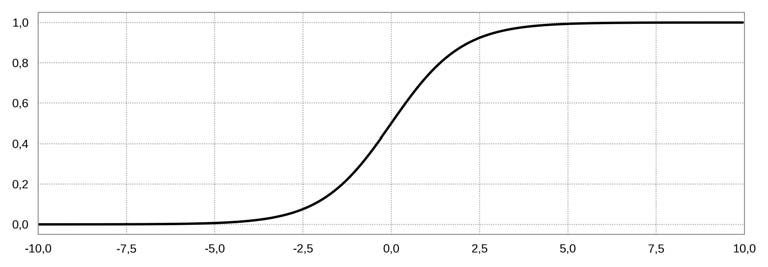
\includegraphics[scale=0.8]{sigmoid.png}
    \caption{Сигмоида}
    \label{fig:sigmoid}
\end{figure}

Обучить этот прецептрон также не составляет труда. Просто теперь мы будем решать задачу бинарной
классификации, а функция ошибки будет cross-энтропией:

\begin{equation}
 L(w) = -\frac{1}{N}\sum_{i=1}^N(y_i\log\sigma(w^\top x_i) + (1-y_i)\log(1-\sigma(w^\top x_i))).
\end{equation}

Эта функция дифференцируема, значит мы можем сделать градиентный шаг. При этом прецептрон с сигмоидой
реализует логистическую регрессию. Обобщение этой модели можно найти в разделе \ref{subsection:logreg}.

\bigskip
Графическое изображение структуры перцепрона представлено на рис. \ref{fig:neuron}, \textit{a}.

\begin{figure}[ht]
    \centering
    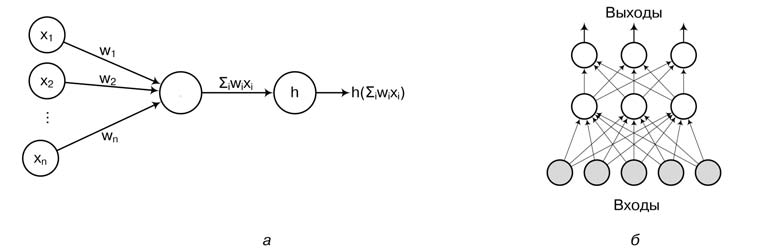
\includegraphics[scale=0.8]{neuron.png}
    \caption{(a) граф вычислений перцептрона; (б) полносвязная нейронная сеть с одним скрытым слоем.}
    \label{fig:neuron}
\end{figure}

На  рис. \ref{fig:neuron}, \textit{б} изображена несложная нейронная сеть, на ее примере покажем как можно векторизовать вычисления в слое нейронов с применением функции активации.

\bigskip
Пусть у нас в слое $k$ нейронов с весами $w_1, w_2, \ldots, w_k$, $\quad w_i = (w_{i1}, \ldots, w_{in})^\top$, на вход вектор $x = (x_1, x_2, \ldots, x_n)^\top$. В результате получим выход $y_i = f(w_i^\top x)$, где $f$ --- функция активации. Эти вычисления можно представить в векторной форме:

\begin{equation*}
\begin{pmatrix}
   y_1 \\
   \ldots \\
   y_k
\end{pmatrix} = y = f(Wx) =
\begin{pmatrix}
   f(w_1^\top x)\\
   \ldots \\
   f(w_k^\top x)
\end{pmatrix}\text{, где } W =
\begin{pmatrix}
   w_1 \\
   \ldots \\
   w_k
\end{pmatrix} =
\begin{pmatrix}
   w_{11} & \ldots & w_{1n}\\
   \ldots &  & \ldots\\
   w_{kk} & \ldots & w_{kn}\\
\end{pmatrix}.
\end{equation*}


% \subsubsection{Функции активации}

Обычно в нелилинейных неронах примемяется сигмоида \ref{eq:sigma}, о которой писалось выше. Но существуют и
другие функции активации, например, $\text{ReLU} = max(0, x)$. Чтобы понять, как она появилась рассмотрим
сумму бесконечного ряда сигмоид, каждая из которых смещена на единицу относительно предыдущей:

\begin{equation*}
 f(x) = \sigma(x+\frac{1}{2} + \sigma(x-\frac{1}{2} + \sigma(x-\frac{3}{2}) + \ldots
\end{equation*}

$f(x)$ можно представить в виде интегала:

\begin{equation*}
 \int_\frac{1}{2}^\infty \sigma(x+\frac{1}{2}-y)dy,
\end{equation*}

Его значение можно приюблизить единичными прямоугольниками:

\begin{equation*}
\begin{aligned}
  \sum_{i=0}^\infty \sigma(x+\frac{1}{2}-i) & \approx \int_\frac{1}{2}^\infty \sigma(x+\frac{1}{2}-y)dy = \\
  & = \left[-\log (1+e^{x+\frac{1}{2}-y})\right]^{y=\infty}_{y=\frac{1}{2}} = \log (1+e^x),
\end{aligned}
\end{equation*}

а это в точности интеграл от сигмиоды:

\begin{equation*}
 \int \sigma (x) dx = \log(1+e^x) + C.
\end{equation*}

Получается бесконечный ряд сигмоид гораздо более выразительная функция активации и это почти тоже самое что и
$\log(1+e^x)$



% Это приближение к ф-ии log(1+e^x) (SoftPlus), которая получается из суммы бесконечного ряда сигмоид со
смещением на 1/2 и тд. Это дает возможность отличать сильно активированные нейроны от слабо активированных.
Но считать производную такой функции очень накладно, поэтому ее приближение -- хороший компромисс. Существуют
еще разные модификации ReLU, например, PReLU или LReLU. В целом она показала лучшую эффективность по сравнению
с сигмоидой и tanh, следовательно используется повсеместно.
%
% SoftMax или нормализованная экспонента. Она нужна чтобы обобщить функцию ошибки для задач классификации,
где классов больше 2-х. Ее удобно использовать на последних слоях нейронной сети, чтобы преобразовать выход в
<<вероятность>>.










































\subsubsection{Распределенные представления слов word2vec}

Подход к обучению моделей распределенных представлений слов был описан в работе Йошуа Бенджи с соавторами
\cite{Bengio}, которая была продолжена в \cite{Zhou}. Идея подхода описанного в \cite{Bengio} основанна на
задаче построения языковой модели, процесс обучения выглядит так:

\bigskip
\begin{itemize}
 \item всем токенам из словаря $i \in V$ ставят в соответствие вектор признаков $w_i$ размерности $d$ ($w_i
\in \mathds{R}^d$). Стандартным значением $d$ является 300;

 \item теперь можно определить вероятности для каждого токена $i$, что он появится в контексте $c_1, \ldots,
c_n$. Для этого определим функцию от векторов признаков $w$:

 \begin{equation}
  \hat{p}(i|c_1, \ldots, c_n) = f(w_i, w_{c_1}, \ldots, w_{c_n}; \theta),
 \end{equation}

 где $w_{c_1}, \ldots, w_{c_n}$ --- векторы признаков токенов из контекста, a $f$ --- фунция с параметрами
$\theta$, которая принимает векторы признаков;

 \item максимизируя логарифм правдоподобия большого корпуса текстов можно обучить векторы признаков $w$ и
параметры $\theta$

 \begin{equation}
  L(W, \theta) = \frac{1}{K}\sum_t \log{f(w_k, w_{k-1}, \ldots, w_{k-n+1}; \theta) + R(W, \theta)},
 \end{equation}

 где $K$ размер окна контекста, а $R(W, \theta)$ --- регуляризация.

\end{itemize}

\bigskip
Для получения функции $f$ можно использовать нейронную сеть. Модель word2vec строится на описании
нейросетевой модели, предложенной в \cite{Bengio}. Она была разработана Томасом Миколовым с соавторами и
опубликована в работах \cite{Mikolov:1, Mikolov:2}, причем в двух вариациях:

\bigskip
\begin{itemize}
 \item CBOW (Continious Bag Of Words) --- по контексту восстановить слово;
 \item skip-gram --- восстановить контекст в зависимости от слова;
\end{itemize}

\bigskip
Архитектура word2vec представляет собой полносвязную нейронную сеть с одним скрытым слоем рис.
\ref{fig:word2vec}.

\begin{figure}[ht]
    \centering
    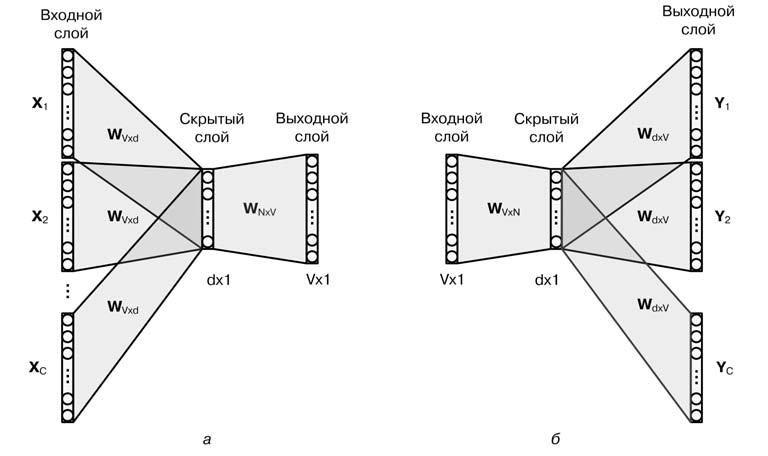
\includegraphics[scale=0.8]{word2vec.png}
    \caption{(a) CBOW; (б) skip-gram.}
    \label{fig:word2vec}
\end{figure}

% !! смещение
Принцип работы модели CBOW \cite{Nikolenko} рис. \ref{fig:word2vec}, \textit{а}  выглядит так:

\bigskip
\begin{itemize}
 \item на вход сети подаются one-hot вектора размерности $V$, где V --- это размер словаря;
 \item скрытый слой --- это матрица $W$ размерности $V\times d$, которая переводит наши представления слов в
$d$ - мерное пространство;
 \item на выходе для каждого слова в словаре берем среднее всех полученных векторов и получаем оценку $u_j$,
где $j = 1, \ldots, V$.
\end{itemize}

\bigskip
Чтобы найти апострериорное распределение модели, просто вычисляем softmax:

\begin{equation}
 \hat{p}(i|c_1, \ldots, c_n) = \frac{\exp{u_j}}{\sum_{j'=1}^V \exp{u_{j'}}}.
\end{equation}

Для аппроксимации апостериорным распределением распределения данных используем loss-функцию для одного окна:

\begin{equation}
 L = -\log{p(i|c_1, \ldots, c_n)} = - u_j + \log{\sum_{j'=1}^{V} \exp{u_{j'}}}.
\end{equation}

Принцип работы модели skip-gram рис. \ref{fig:word2vec}, \textit{б} полностью противоположный. До этого мы
усредняли контекст, чтобы получить среднее слово в окне, а теперь будем предсказывать слова контекста исходя
из центрального слова. На выходе мы получаем $K-1$ мультиномиальных распределений (центральное слово не
учитывается):

\begin{equation}
 \hat{p}(c_k|i) = \frac{\exp{u_{kc_k}}}{\sum_{j'=1}^V \exp{u_{j'}}},
\end{equation}

loss-функция для окна размера K выглядит так:

\begin{equation}
 L = -\log{p(c_1, \ldots, c_n|i)} = - \sum_{k=1}^{K} u_{kc_k} + n\log{\sum_{j'=1}^{V} \exp{u_{j'}}}.
\end{equation}

Возникает вопрос, как же обучить такую модель? Этот процесс хорошо описан в докладе Голдберга и его соавторов
\cite{Goldberg}.

\bigskip
Подробно разберем модель skip-gram для корпуса документов $D$. Нашей задачей стоит нахождение оптимальных
параметров модели $\theta$, чтобы максимизировать функцию правдоподобия:

\begin{equation} \label{eq:likelyhood}
 L(\theta)=\prod_{i\in D}\left(\prod_{c\in C(i)} p(c|i;\theta)\right) = \prod_{(i,c)\in D}p(c|i;\theta),
\end{equation}

где $C(i)$ --- множество контекстных слов внутри окна вокруг центрального слова $i$. Вероятность $p(c|i;\theta
)$ определяется, как softmax-функция, зависящая от всех возможных векторов контекста.

\begin{equation} \label{eq:generalSoftmax}
 p(c|i;\theta) = \frac{\exp{\tilde{w}_c^\top w_i}}{\sum_{c'} \exp{\tilde{w}_{c'}^\top w_i}},
\end{equation}

где $\tilde{w}_c$ --- вектор признаков слова из контекста $c$, который отличается от $w_i$. Для каждого слова
$i$ надо обучить два вектора признаков $w_i$ и $\tilde{w}_i$, в первом случае это слова выступает в качестве
центрального, во втором в качестве контекстного.

\bigskip
Эта особенность обучения, когда мы берем два разных вектора одного и того же слова вместо одного, описана в
\cite{Goldberg}. И мотивирована тем, что слова редко встречаются в контексте себя самих. Вот, например, слово
<<мотивация>> вряд ли можно встретить в контексте другого слова <<мотивация>>, под это правило попадают почти
все слова. Поэтому в процессе обучения модель сведет вероятности $p(i|i, \theta)$ к нулю. А если вектора
контекста и центрального слова будут равны нулю, то норма вектора $|w_i| = w_i^\top w_i$ тоже будет равняться
нулю, а это очень не желательно. Поэтому для каждого слова мы обучаем два разных вектора.

\bigskip
Теперь выразим максимум функции правдоподобия для всего корпуса через логарифм \ref{eq:likelyhood} и
\ref{eq:generalSoftmax}:

\begin{equation}
\begin{aligned}
 \argmax_{\theta} \prod_{(i,c)\in D} & p(c|i;\theta) = \argmax_{\theta} \sum_{(i,c)\in D}\log{p(c|i;\theta)} =
\\
 & = \argmax_{\theta} \sum_{(i,c)\in D} \left(\exp{\tilde{w}_c^\top w_i} - \log{\sum_{c'}
\exp{\tilde{w}_{c'}^\top w_i}}\right).
\end{aligned}
\end{equation}

Оптимизируя данную функцию мы получаем хорошее распределенное представление слов. Но для этого нужно решить
сложнейшую задачу: суммировать скалярные произведения всех возможных слов и их контекста $\sum_{c'}
\tilde{w}_c^\top w_i$ при том, что размер словаря может достигать миллионов.

\bigskip
Чтобы уменьшить количество вычислений Миколов с соавторами \cite{Mikolov:2} предложили элегантный метод:
negative sampling. Нам не нужно считать всю сумму $\sum_{c'} \tilde{w}_c^\top w_i$, а только случайно выбрать
несколько ее элементов в качестве отрицательных примеров (примеры в которых слово не находится в определенном
контексте) и обновить только их. Т.е. теперь нам нужно посчитать только небольшую сумму $\sum_{c' \in D'}
\tilde{w}_c^\top w_i$, где $D'$ --- случайное подмножество отрицательных примеров.

\bigskip
По сути negative sampling --- это тоже правдоподобие, но другого события. Пусть у нас есть слово $i$ и его
контекст $c$, наша задача максимизировать вероятность $p((i,c) \in D; \theta)$, параметризированную вектором
$\theta$, т.е. правдоподобие появления пары $(i,c)$:

\begin{equation}
 \argmax_{\theta} \prod_{(i,c)\in D} p((i,c)\in D;\theta) = \argmax_{\theta} \sum_{(i,c)\in D} \log{
p((i,c)\in D;\theta)}.
\end{equation}

Выразим $p((i,c)\in D;\theta)$ через softmax. Но так как это бинарное событие, то заменим softmax сигмоидой
$\sigma (x) = \frac{1}{1+\exp{(-x)}}$:

\begin{equation}
 p((i,c)\in D;\theta) = \frac{1}{1+\exp{(-\tilde{w}_c^{\top} w_i)}}
\end{equation}

Максимизируем логарифм правдоподобия:

\begin{equation} \label{eq:negLikelyhood}
\begin{aligned}
 \argmax_{\theta} \sum_{(i,c)\in D} & \log{p((i,c)\in D;\theta)} = \\
 & = \argmax_{\theta} \sum_{(i,c)\in D} \log{\frac{1}{1+\exp{(-\tilde{w}_c^{\top} w_i)}}}.
\end{aligned}
\end{equation}

Из \ref{eq:negLikelyhood} видно, что оптимальное значение логарифма будет получено при максимальном значении
скалярного произведения $\tilde{w}_c^{\top} w_i$. Сделаем равные векторы с большой нормой и можно без проблем
получить правдоподобие почти равное единице. Подвох заключается в том, что модель обучается на данных для
бинарной классификации, но мы рассматриваем только набор состоящий из положительных примеров. Классификатор,
который всегда предсказывает <<да>> --- плохой. Поэтому имеет смысл добавить отрицательных примеров, просто
случайно выбирая слова и контекст, которых нет в данных. После того, как мы получим набор отрицательных
данных, максимизация правдоподобия будет выглядеть так:

\begin{equation} \label{eq:generalLikelyhood}
 \argmax_{\theta} \prod_{(i,c)\in D} p((i,c)\in D;\theta) \prod_{(i,c)\in D'} p((i',c')\notin D;\theta)
\end{equation}

Выразим в \ref{eq:generalLikelyhood} пару $(i,c) \in D$:

\begin{equation}
\begin{aligned}
 & \argmax_{\theta} \prod_{(i,c)\in D} p((i,c)\in D;\theta) \prod_{(i,c)\in D'} 1-p((i',c')\in D;\theta) = \\
 = & \argmax_{\theta} \left[\sum_{(i,c)\in D} \log{p((i,c)\in D;\theta)} + \sum_{(i,c)\in D'} \log{(
1-p((i',c')\in D;\theta))} \right] = \\
 = & \argmax_{\theta} \sum_{(i,c)\in D} \left[\log{\frac{1}{1+\exp{(-\tilde{w}_c^{\top} w_i)}}} +
\sum_{(i,c')\in D'} \log{\frac{1}{1+\exp{(\tilde{w}_{c'}^{\top} w_i)}}} \right] = \\
 = & \argmax_{\theta} \sum_{(i,c)\in D} \left[\log\sigma(\tilde{w}_c^{\top} w_i) + \sum_{(i,c')\in D'}
\log\sigma(-\tilde{w}_{c'}^{\top} w_i)\right]
\end{aligned}
\end{equation}

Получили формулу для negative sampling из \cite{Mikolov:2}. Значит мы для каждого окна случайно берем
несколько отрицательных примеров $D'$ и делаем градиентный шаг для loss-функции:

\begin{equation}
 L = \log\sigma(\tilde{w}_c^{\top} w_i) \sum_{(i,c')\in D'} \log\sigma(-\tilde{w}_{c'}^{\top} w_i)
\end{equation}

Аналогичные рассуждения можно провести для модели CBOW.

% ++ можно добавить матричный подход

\subsubsection{ELMo}

Создание этой модели породило новую эру распределенных представлений слов. Word2vec показал, что с помощью векторов можно представлять слова в виде, который может передавать их семантику или смысловые отношения (т.е. способность различать схожие и противоположные по смыслу слова или находить параллели в отношениях таких словарных пар, как <<Женщина - Мама>> и <<Транспорт - Повозка>>), а также синтаксические или грамматические отношения (например, определять, что отношение между <<Красиво и Красивый>>) \cite{elmoru}.

\bigskip
Почему бы не сделать распределенное представление слов на основе контекста, в котором оно стоит? Чтобы передавать не только значение слова, но и контекстуальную информацию. Так появились контекстуализированные распределенные представления слов (contextualized word-embeddings)

\bigskip
Способность понимать язык ELMo получила после обучения предсказыванию нового слова в последовательности слов. Эта задача, называется языковым моделированием (language modeling).

\bigskip
В \cite{elmoen} показано, что двунаправленная языковая модель (biLM) является основой для ELMo. В то время как входные данные представляют собой последовательность $n$ слов $(x_1, \ldots, x_n)$ языковая модель предсказывает условную вероятность следующего слова:

\bigskip
В прямом проходе последовательность содержит слова перед целевым словом:

\begin{equation*}
  p(x_1, \ldots, x_n) = \prod_{i=1}^n p(x_i| x_1, \ldots, x_{i-1}).
\end{equation*}

\bigskip
При обратном проходе последовательность содержит слова после целевого слова:

\begin{equation*}
  p(x_1, \ldots, x_n) = \prod_{i=1}^n p(x_i| x_{i+1}, \ldots, x_n).
 \end{equation*}

\bigskip
Предсказания в обоих направлениях моделируются многослойными LSTM ячейками со скрытыми состояниями $\overrightarrow{h}_{i,l}$ и $\overleftarrow{h}_{i,l}$ и для входного слова $x_i$ на уровне слоя $l = 1, \ldots, L$. Скрытое состояние последнего слоя $h_{i,L} = [\overrightarrow{h}_{i,L}; \overleftarrow{h}_{i,L}$ используется для вывода вероятностей по словам после нормализации softmax. Эти скрытые состояния разделяют слой распределенного представления слов и слой softmax, которые параметризованы $\Theta_e$ и $\Theta_s$ соответственно.

\begin{figure}[ht]
    \centering
    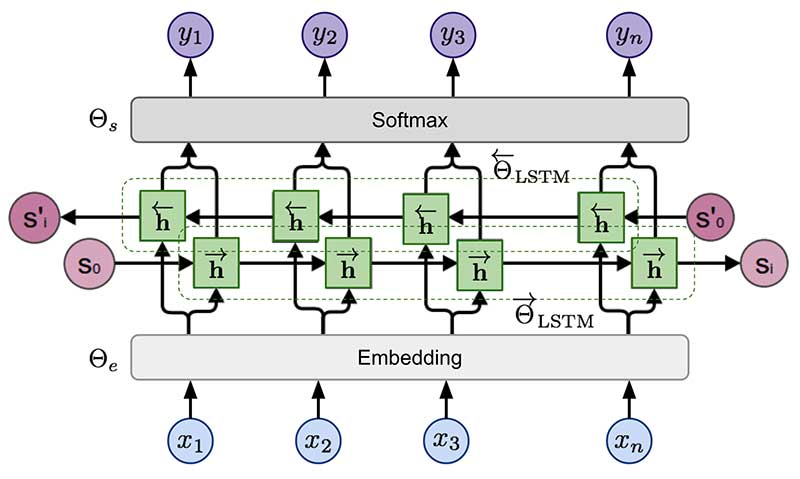
\includegraphics[scale=0.5]{ELMo.jpg}
    \caption{Базовая модель biLSTM ELMo. Источник: \cite{elmopic}}
    \label{fig:elmo}
\end{figure}

\bigskip
Процесс обучения модели --- максимизация логарифма правдоподобия для истиных слов в обоих направлениях:

\begin{equation*}
\begin{aligned}
 \lh (x) = \argmax \sum_{i=1}^n \bigg[ & \log p(x_i| x_1, \ldots, x_{i-1}|\Theta_e,\overrightarrow{\Theta}_{LSTM}, \Theta_s) + \\
 + & \log p(x_i| x_{i+1}, \ldots, x_n| \Theta_e,\overleftarrow{\Theta}_{LSTM}, \Theta_s)\bigg]
\end{aligned}
\end{equation*}








\subsection{Классификация}


\subsubsection{Анализ качества классификации}

Для оценки качества классификации используется Macro\,F1-мера --- нормализованное по всем классам среднее гарманическое метрик $P$ и $R$:

    \begin{equation*}
    \text{Macro F1} =  \frac{1}{n}\sum_{i=1}^n 2\frac{P_i\times R_i}{P_i + R_i} = \frac{1}{n}\sum_{i=1}^n
\text{F1}_i,
    \end{equation*}

где $P$ --- точность и $R$ --- полнота.

\bigskip\noindent
Ее преймущество в том, что она не учитывает дисбаланс классов.

\begin{definition}
 Точностсь (\textit{precision}) --- показывает долю объектов, которые классификатор определил, как принадлежащие действительно правильному классу.
\end{definition}

\begin{equation*}
 P = \frac{TP}{TP + FP},
\end{equation*}

\bigskip
где $TP$ --- те метки которые мы ожидали и получили, $FP$ --- те метки которые мы не ожидали, но получили на выходе.

\begin{definition}
 Полнота (recall) --- показывает какую долю объектов из всего множества конкретного класса калассификатор определил верно.
\end{definition}

\begin{equation*}
 R = \frac{TP}{TP + FN},
\end{equation*}

\bigskip
где $FN$ --- те метки которые мы ожидали, но не получили на выходе.




\subsubsection{Кросс-валидация}

Методом оценки аналитической модели и её поведения на независимых данных является перекрестная проверка k-fold cross validation, при $k$ = 10.


















\subsubsection{Логистическая регрессия}
\label{subsection:logreg}

Логистическая регрессия --- классическая дискриминативной линейная модель классификации. Дискриминативная
значит, что нас интересует $P (y = k | x)$, а не совместное распределение $p (x, y)$. Свое начало она берет из
расстояния Кульбака-Лейблера. Оно задается формулой:

\begin{equation}
 KL(P||Q) = \int\log\frac{dP}{dQ}dP,
\end{equation}

, где $P$ --- истинное распределение, а $Q$ --- приближенное. Для дискретного случая:

\begin{equation}
 KL(P||Q) = \sum_{y} p(y)log\frac{p(y)}{q(y)},
\end{equation}

а если раскрыть получаем:

\begin{equation}
\begin{aligned}
 KL(P||Q) & = \sum_y p(y)\log\frac{p(y)}{q(y)} = \\
 & = \sum_y p(y) \log p(y) - \sum_y p(y) \log q(y) = - H(p) + H(p,q),
\end{aligned}
\end{equation}

, где $H(p)$ ---  энтропия распределения $p$, a $H(p, q)$ --- наша кросс энтропия. Из этой суммы видно, что
нам нужно минимизировать $H(p, q)$. Для бинарной классификации loss-функция будет выглядеть так:

\begin{equation} \label{eq:logLoss}
 L(w)= H(p_{data}, q(w)) = -\frac{1}{N}\sum_{i=1}^N(y_i\log\hat y_i(w) + (1-y_i)\log(1-\hat y_i(w)))
\end{equation}

где $p_{data}$ --- распределение наших данных, $q(w)$ --- апостериорное распределение,  $\hat y_i(w)$ ---
оценка вероятности при входных параметрах $w$ и $y_i$ --- истинное предсказание. Два слагаемых мы получаем,
т.к. события несовместные. Например, в тексте говорится о кошечках или о собачках, события появления кошечки
или собачки несовместные, т.е. $p(\text{кошечки}) = 1 - p(\text{собачки})$. Если мы предсказываем кошечку (1),
как абсолютный 0 или собачку (0), как 1, то ошибка будет бесконечной из первого и второго слагаемых
соответственно -- это не допустимо.

Перед тем, как перейти к нескольким классам, рассмотрим сначала задачу классификации с Байейсовской точки
зрения: определим для каждого класса $C_k$ плотность $p(x|C_k)$ и какие-то априорные распределения $p(C_k)$
(пускай это будут размеры классов, т.е. мы ничего не знаем о примере, но предполагаем с какой вероятностью он
относится к конкретному классу) и найдем $p(C_k|x)$. Для двух классов:

\begin{equation}
\begin{aligned}
 p(C_1|x) & = \frac{p(x|C_1)p(C_1)}{p(x|C_1)p(C_1)+p(x|C_2)p(C_2)} = \\
 & = 1/\frac{(p(x|C_1)p(C_1)+p(x|C_2)p(C_2))}{p(x|C_1)p(C_1)} = \\
 & = 1/(1+\frac{p(x|C_2)p(C_2)}{p(x|C_1)p(C_1)}) = \frac{1}{1+e^{-a}} = \sigma (a),
\end{aligned}
\end{equation}

где

\begin{equation}
 a = \ln\frac{p(x|C_1)p(C_1)}{p(x|C_2)p(C_2)},\qquad \frac{1}{1+e^{-a}} = \sigma (a).
\end{equation}

Используя логистическую регрессию мы делаем предположение о виде аргумента сигдмоиды $a$ --- это будет
скалярное произведение вектора признаков на вектор данных: $a = w_\top x$. Cигмоида переводит результат
вычисления этой линейной функции на отрезок $[0;1]$ и как результат мы получаем апостериорную вероятность
первого или второго классов:

\begin{equation}
 p(C_1|x) = y(x) = \sigma (w_\top x),\qquad p(C_2|x) = 1-p(C_1|x),
\end{equation}

чтобы обучить эту модель мы можем просто оптимизировать правдоподобие по $w$.

Для набора ${x_n, t_n}$, где $x_n$ -- входы, а $t_n \in \{0;1\}$ -- соответствующие метки классов, получается
такое правдоподобие:

\begin{equation}
 p(t|w) = \prod_{n=1}^N y_n^{t_n}(1-y_n)^{1-t_n},\quad\text{где}\quad y_n = p(C_1|x_n).
\end{equation}

И теперь мы, максимизируя логарифм вероятности, ищем наилучшие параметры функции правдоподобия для этого можно
использовать различные оптимизаторы.

\begin{equation}
 \lh (w) = -\ln p(t|w) = -\sum_{n=1}^N[t_n \ln y_n + (1-t_n) \ln (1-y_n)].
\end{equation}

Теперь можно легко обобщить задачу на несколько классов. Только вместо сигмоиды будем использовать softmax
функцию. Для $K$ классов получаем:

\begin{equation}
 p(C_k|x) = \frac{p(x|C_k)p(C_k)}{\sum_{j=1}^K p(x|C_j)p(C_j)} = \frac{e^{a_k}}{\sum_{j=1}^K e^{a_j}},
\end{equation}

где количество аргументов $a_k = \ln p(x|C_k)p(C_k)$ равняется количеству классов. Функция правдоподобия почти
не изменилась. Пусть на вход метки класса подаются в формате one-hot векторов, тогда для набора векторов $T =
{t_n}$ функция правдоподобия выглядит следующим образом:

\begin{equation}
 p(T|w_1,\ldots,w_K) = \prod_{n=1}^N \prod_{k=1}^K p(C_k|x_n)^{t_{nk}} = \prod_{n=1}^N \prod_{k=1}^K
y_{nk}^{t_{nk}}.
\end{equation}

, где $y_{nk} = y_k(x_n)$. Опять переходим к логарифму и получаем функцию максимального правдоподобия для $K$
классов:

\begin{equation}
 \lh (w_1,\ldots,w_K) = -\ln p(T|w_1,\ldots,w_K) = \sum_{n=1}^N \sum_{k=1}^K t_{nk}\ln y_{nk}.
\end{equation}


\subsubsection{Метод опорных ввекторов}
















\subsubsection{Случайный лес}


























\section{ПРАКТИЧЕСКАЯ ЧАСТЬ}
\vspace{-1.3cm}

\subsection{Используемые инструменты}

\begin{itemize}
 \item Python 3


 \item NumPy


 \item Pandas


 \item Matplotlib


 \item Pymorphy2


 \item Razdel


 \item Scikit-learn


 \item TensorFlow


 \item JavaScript


 \item HTML и CSS
\end{itemize}


% \begin{itemize}
%  \item Python 3;
%  \begin{itemize}
%   \item nltk;
%   \item Pymorphy2;
%   \item NumPy;
%   \item Pandas;
%   \item Razdel;
%   \item Matplotlib;
%   \item Scikit-learn;
%   \item TensorFlow.
%  \end{itemize}
%
%  \item JavaScript;
%  \item HTML и CSS.
% \end{itemize}


\subsection{Сбор данных}


Самым главным этапом перед созданием моделей-классификаторов является сбор данных, этот процесс включает в себя несколько основных этапов:

\bigskip
\begin{itemize}
 \item обработка и подготовка текстов;
 \item разметка текстов;
 \item обработка полученных результатов.
\end{itemize}

\subsubsection{Обработка и подготовка текстов}

В качестве основного текста для разметки был взят роман Михаила Афанасьевича Булгакова <<Мастер и Маргарита>>.

\bigskip
Обработка документа:

\bigskip
\begin{enumerate}
\item произведение было очищено от нежелательных подстрок регулярными выражениями;
\item разделено на тексты по символу перевода строки <<\textbackslash n>>;
\item из полученных текстов восстановлена прямая речь;
\item тексты содержащие больше 52 слов разделены с использованием библиотеки <<razdel>>.
\end{enumerate}

\bigskip
Формирование заданий:

\bigskip
\begin{itemize}
 \item для разметки выделены тексты от 5 до 52 слов;
 \item для каждого текста определен контекст:  не менее 40 слов перед и не менее 15 после текста.
\end{itemize}



\subsubsection{Разметка текстов}

Чтобы приступить к разметке сначала нужно определить множество меток классов, для этого обратимся к истории создания эмоциональных моделей ведущими профессорами в области изучения эмоций. В 1980 году Роберт Плутчик в своей работе \cite{Plutchik} определил колесо эмоций рис. \ref{fig:plutchik}. Данная модель была взята за основу и дополнена моделью Пола Экмана, которую он описал в работе \cite{Ekman2004} 2004 года и обновил в статье \cite{Ekman2011} 2011 года.

\begin{figure}[ht]
    \centering
    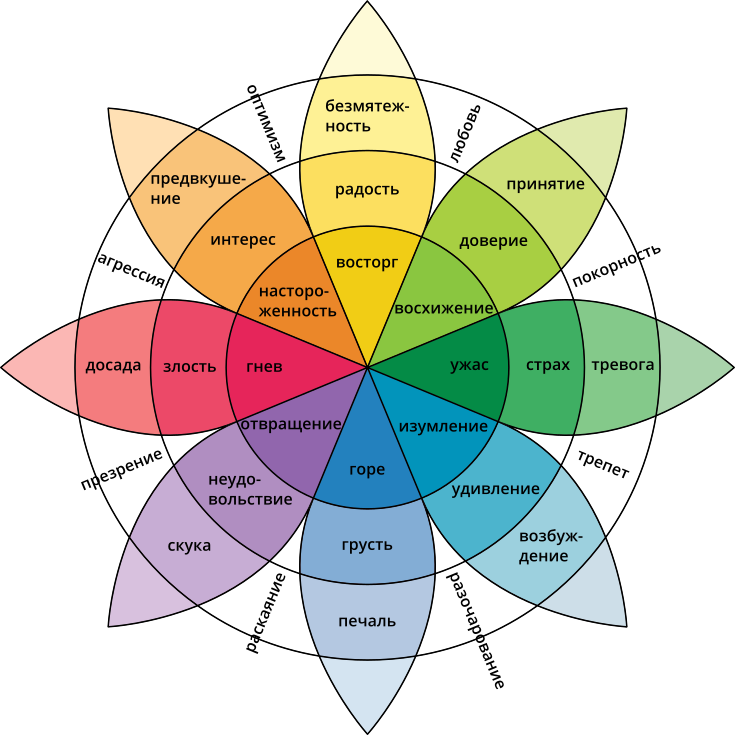
\includegraphics[scale=0.5]{plutchik.png}
    \caption{Колесо эмоции Роберта Плутчика}
    \label{fig:plutchik}
\end{figure}

В результате получилось множество, состоящее из 9 основных эмоций и их производных, дополненное нейтральным классом:

\bigskip
\begin{itemize}
\item \textbf{Злость} (anger) --- желание выразить агрессию или причинить зло, общая для обеих моделей.\\
Может проявляться в словах, мимике, поступках.
Примеры: злость на оскорбление, на несправедливость, злость на плохое отношение.\\
Гнев --- более интенсивная эмоция, досада --- менее.

\item \textbf{Интерес} (anticipation) --- предчувствие важного события, только в модели Плутчика.\\
Проявляется в нетерпении, волнении.
Примеры: ожидание праздника, ожидание начала каникул, ожидание плохой оценки.\\
Настороженность --- более интенсивная, предвкушение --- менее.

\item \textbf{Радость} (joy) --- чувство удовольствия, весёлого настроения и счастья, общая для обеих моделей.\\
Проявляется в смехе, улыбке, ласковом обращении к другим.
Примеры: радость по поводу подарка, общения с другом.\\
Восторг --- более интенсивная, безмятежность --- менее.

\item \textbf{Доверие} (trust) --- ​открытое теплое отношение к чему бы то ни было (другу/животному/миру/...), только в модели Плутчика.\\
Проявляется в уверенности в положительном исходе.
Примеры: доверие другу при встрече с неожиданностями, доверие к собаке, что не укусит, доверие к доктору, что он делает полезные вещи.\\
Восхищение --- более интенсивная, принятие --- менее.

\item \textbf{Страх} (fear) --- состояние перед реальным или предполагаемым бедствием, общая для обеих моделей.\\
Проявляется в волнении, напряжении.
Пример: страх наказания, страх проигрыша, страх попасть в аварию.\\
Ужас --- более интенсивная, тревога --- менее.

\item \textbf{Удивление} (surprise) --- эмоциональная реакция на неожиданную ситуацию, общая для обеих моделей.\\
Удивление может проявляться в хороших и плохих ситуациях.
Примеры: получил плохой отзыв на работу вместо ожидаемого хорошего, директор школы привел в класс собаку, одноклассник вырос на 10 см за лето.\\
Изумление --- более интенсивная, возбуждение --- менее.


\item \textbf{Грусть} (sadness) --- отсутствие радости,​ неудовлетворенность происходящим, отстраненность, общая для обеих моделей.\\
Проявляется в нежелании веселиться с другими, желании заботы и участия.
Примеры: мама уехала в командировку надолго, не покупают собаку или велосипед, никак не дается математика.\\
Горе --- более интенсивная, печаль --- менее.

\item \textbf{Неудовольствие} (disgust) --- эмоциональная реакция на неприятную ситуацию или объект.\\
Проявляется в неприятии человека, любых вещей, ситуаций, общая для обеих моделей.
Примеры: когда сталкиваешься с неприятным запахом, грязными вещами, плохим поведением.\\
Отвращение --- более интенсивная, скука --- менее.

\item \textbf{Презрение} (contempt) --- пренебрежительное отношение к кому-чему-нибудь морально низкому, недостойному, подлому. Презрение связано с чувством превосходства. Также оно может перейти в безразличное отношение к кому-чему-то. Только в модели Экмана.

\item \textbf{Нейтральное} (neutral) --- безэмоциональное повествование.

\end{itemize}

\bigskip
Разметка осуществлялась с помощью краудсорсинговой платформы <<Яндекс.Толока>>.

\begin{definition}
 Краудсорсинг --- это привлечение добровольцев и экспертов для выполнения определенной работы, действующих на добровольной или коммерческой основе.
\end{definition}

Для получения более точной разметки данных были использованы встроенные методы и инструменты контроля качества:

\bigskip
\begin{itemize}
 \item график времени выполнения страницы заданий рис. \ref{fig:task-time} нужен, чтобы видеть на сколько вдумчиво эксперт расставляет метки;
 \item график выполнения заданий рис. \ref{fig:task-accept} показывает сколько выполнено страниц заданий, сколько просрочено и сколько пропущено. По нему можно судить о сложности выполнения задания и использовать эту информацию в процессе формирования новых пулов заданий;
 \item сформирована система правил, которая позволяет контролировать процесс разметки в автономном режиме:
    \medskip
    \begin{itemize}
     \item Eсли пропущенных подряд страниц заданий $\geqslant 10$, то заблокировать на проекте на $2$ дня;
     \item Eсли отправленных страниц заданий $\geqslant 50$, то заблокировать на проекте на $2$ дня;
     \item Минимальное время на страницу заданий --- $250$ сек. Учитывать последних страниц заданий --- $15$. Если количество ответов $\geqslant 5$ и количество быстрых ответов $\geqslant 5$, то заблокировать на проекте на $2$ дня и т.д.
    \end{itemize}
 \item размечены контрольные задания, с их помощью можно отслеживать примерную точность (accuracy), как всего набора данных, так и набора, полученного от одного эксперта;
 \item каждое задание выполняло три различных эксперта (перекрытие x3);
 \item агрегация результатов производилась методом Дэвида-Скина. Он автоматически оценивает для каждого исполнителя $|L|^2$ параметров, где $L$ --- множество возможных различных значений для агрегации и возвращает итоговый ответ и его статистическую значимость.
\end{itemize}


\begin{figure}[ht]
    \centering
    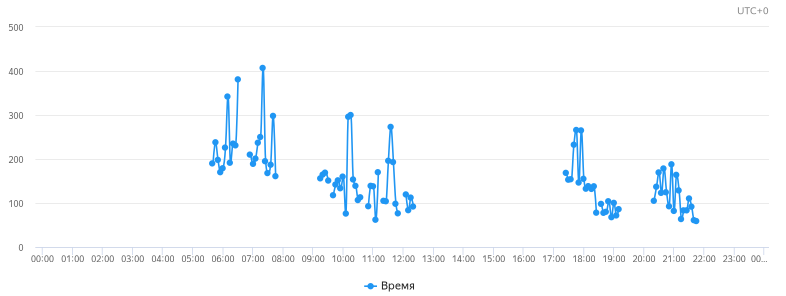
\includegraphics[scale=0.5]{task-time.png}
    \caption{Время выполнения страницы заданий (детализация по 5 минут)}
    \label{fig:task-time}
\end{figure}



\begin{figure}[ht]
    \centering
    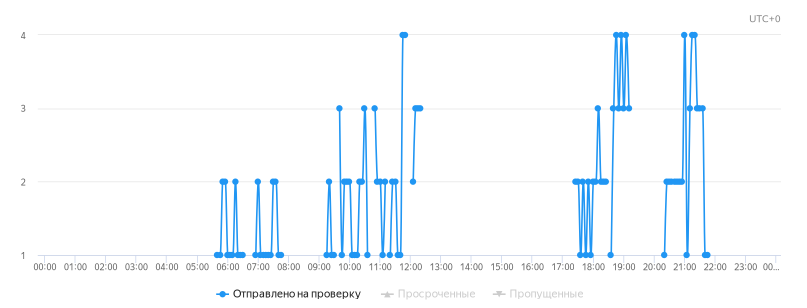
\includegraphics[scale=0.5]{task-accept.png}
    \caption{Выполнение страниц заданий (детализация по 5 минут)}
    \label{fig:task-accept}
\end{figure}

\bigskip
Была разработана форма задания рис. \ref{fig:task}. Каждое задание состоит из трех текстовых блоков. Страница заданий состоит из двух не размеченных заданий и одного контрольного, такое разбиение оптимально для получения качественных результатов. Эксперт должен прочитать каждый текстовый блок и отметить эмоции, которые, по его мнению, описаны в выделенном фрагменте.

\begin{figure}[ht]
    \centering
    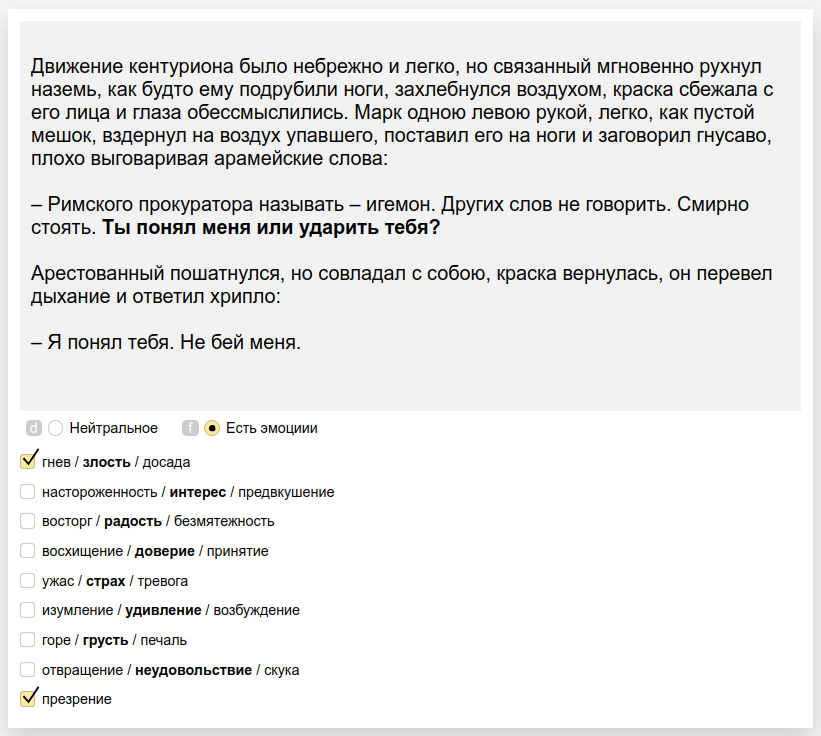
\includegraphics[scale=0.5]{task.png}
    \caption{Форма задания в сервисе <<Яндекс.Толока>>}
    \label{fig:task}
\end{figure}

\bigskip
В результате был сформирован набор данных с таким распределением классов рис. \ref{fig:class_distribution}.



\begin{figure}[ht]
    \centering
    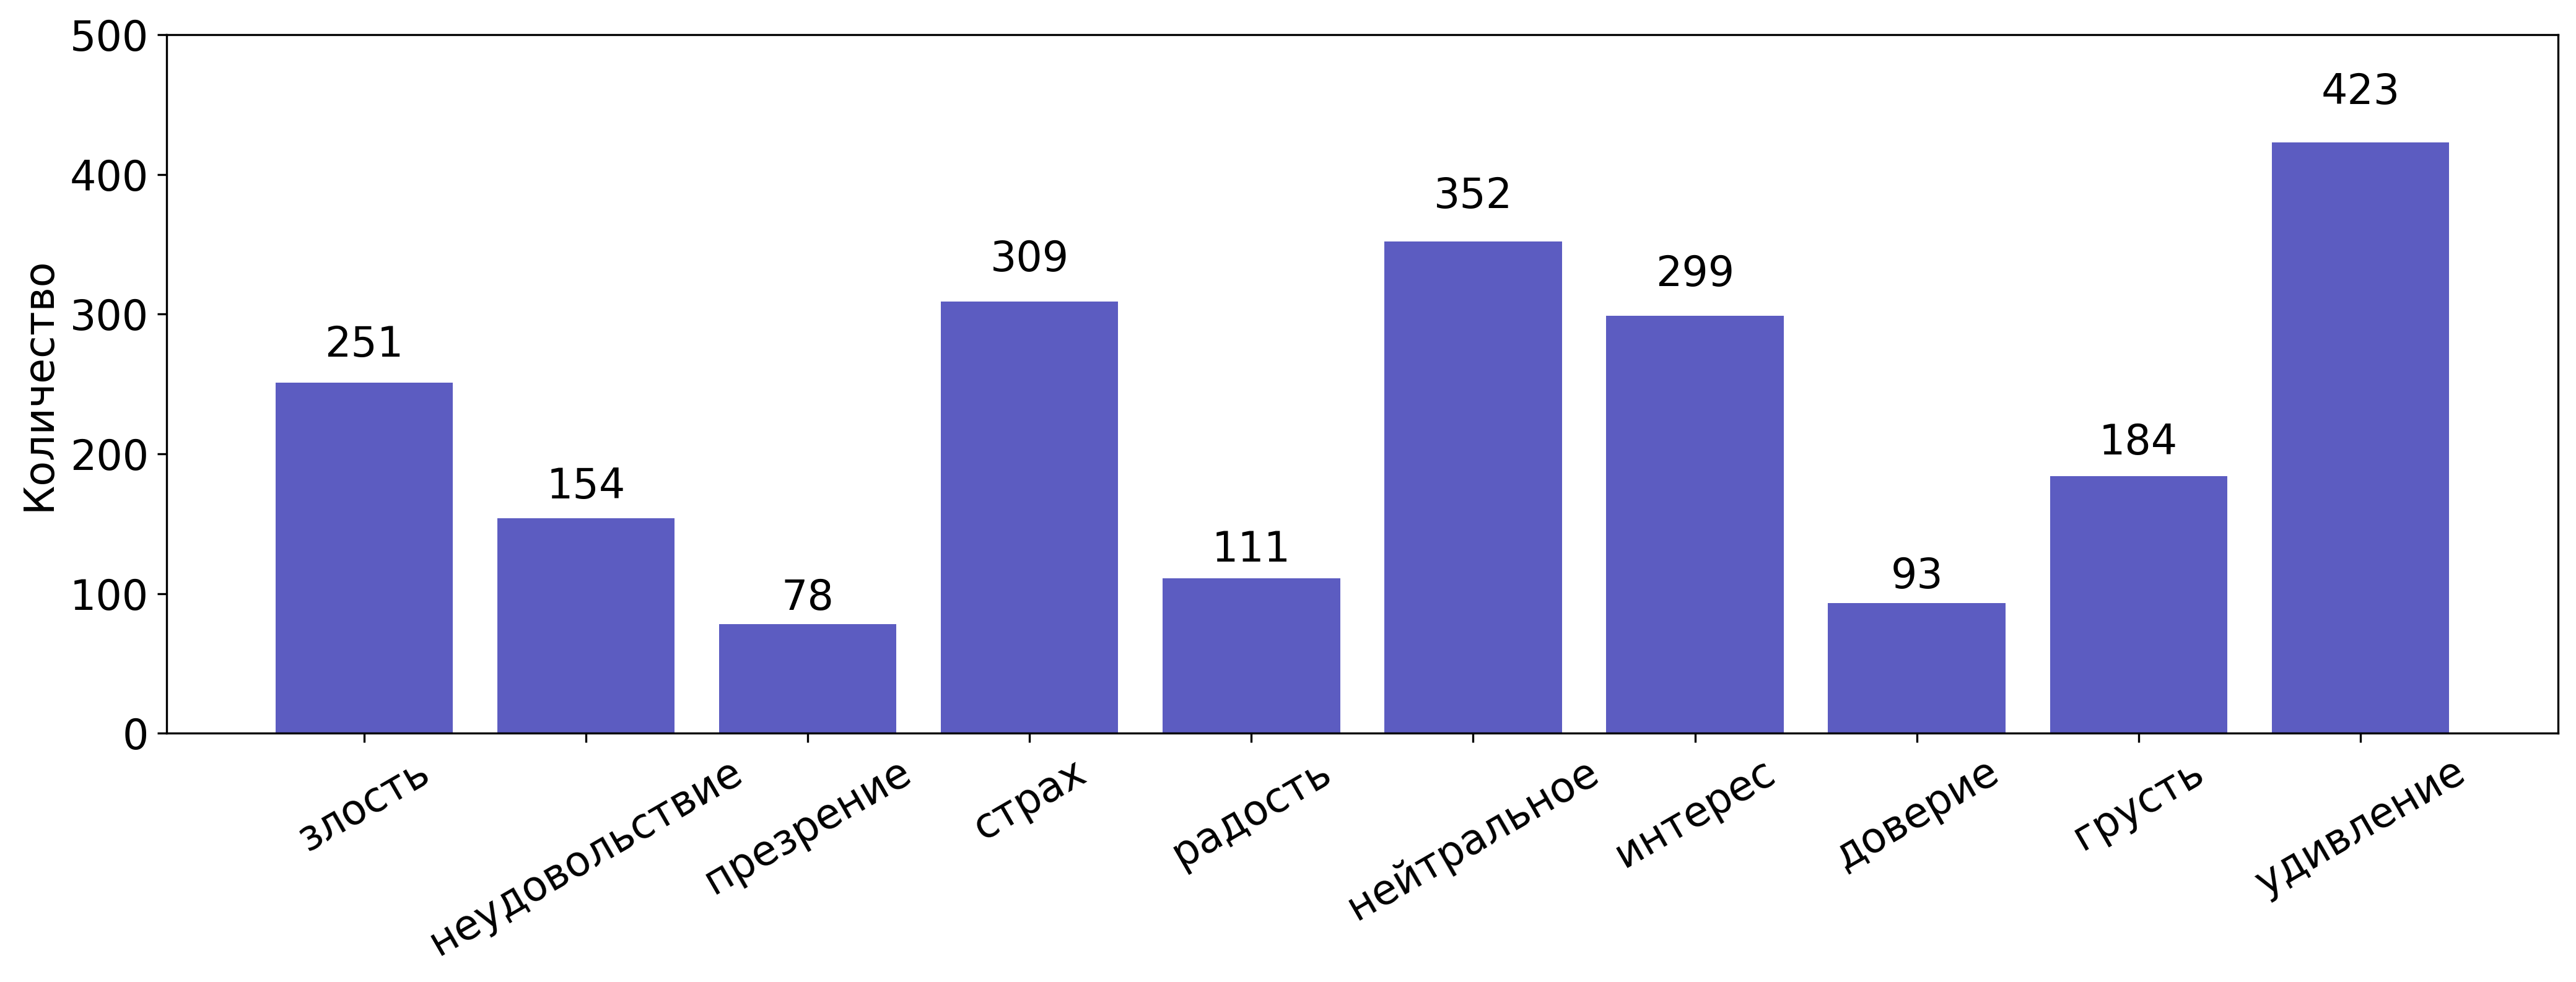
\includegraphics[scale=0.45]{class_distribution.png}
    \caption{Распределение классов в итоговом наборе данных}
    \label{fig:class_distribution}
\end{figure}

\subsection{Модели классификации}
\vspace{-1.3cm}
\subsubsection{Предобработка текстов}

Чтобы работать с текстами, сначала их нужно нормализовать. Этот процесс включает несколько этапов.

\bigskip
\begin{enumerate}
 \item приводим текст к нижнему регистру;
 \item удаляем все <<не слова>> и <<стоп-слова>>;
 \item лемматизируем текст.
\end{enumerate}

\bigskip
Вот пример обработки небольшого текста:

\bigskip
\fbox{Квартира простояла пустой и запечатанной только неделю.} $\to$ \fbox{квартира простаивать пустой запечатывать неделя}


\subsubsection{Представление предложений}


Теперь текст нужно перевести в векторное пространство $R^n$, где $n$ --- размерность признаково пространства используемой модели. Пусть текст $D$ состоит из слов $d \in D$, $f$ --- модель, строящая отображение пространства слов в векторное пространство действительных чисел $f(d) \to R^n$. Тогда текст для классификатора выглядит так:

\begin{equation*}
 \frac{1}{\#D}\sum_{d \in D} f(d) \in R^n
\end{equation*}

В этой работе использованы модели предобученные на корпусе русскоязычных текстов <<Тайга>>:

\bigskip
\begin{itemize}
 \item word2vec \& skip-gram: \textit{tayga\_upos\_skipgram\_300\_2\_2019} ($n = 300$);
 \item ELMo: \textit{tayga\_lemmas\_elmo\_2048\_2019} ($n = 2048$).
\end{itemize}

\bigskip
Особенность применения ELMo заключается в том, что берется среднее значение всех слоев для каждого слова.

\subsection{Архитектура моделей классификации}

Для классификации были выбраны алгоритмы классического машинного обучения:

\bigskip
\begin{itemize}
 \item случайный лес (Random Forest);
 \item логистическая регрессия (Logistic Regression);
 \item метод опорных векторов (Support Vector Machine).
\end{itemize}

\bigskip\noindent
Схематично модели классификации представлены на рис. \ref{fig:models}.

\begin{figure}[ht]
    \centering
    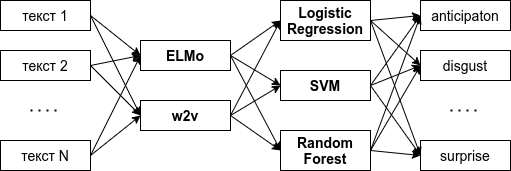
\includegraphics[scale=0.6]{models.png}
    \caption{Архитектура моделей классификации}
    \label{fig:models}
\end{figure}


\subsection{Эксперименты}

\noindent
Для эмоциональной модели Роберта Плутчика результаты представлены в таблице \ref{tab:plutchik}.

\bigskip
\begin{table}[ht]
\caption{Значения Macro F1 меры}
\label{tab:plutchik}
\centering
\begin{tabular}{|c|c|c|c|c|}
\hline Macro F1 & \textbf{log reg} & \textbf{SVM} & \textbf{random forest} & \textbf{tuned random forest} \\
\hline \textbf{w2v} & 0.21519548 & 0.27992996 & 0.23415391 & 0.23932876 \\
\hline \textbf{ELMO} & 0.25900211 & 0.32828541 & 0.31197309 & 0.43861588 \\
\hline
\end{tabular}
\end{table}


\noindent
Для эмоциональной модели Пола Экмана --- в таблице \ref{tab:ekman}.


\bigskip
\begin{table}[ht]
\caption{Значения Macro F1 меры}
\label{tab:ekman}
\centering
\begin{tabular}{|c|c|c|c|c|}
\hline Macro F1 & \textbf{log reg} & \textbf{SVM} & \textbf{random forest} & \textbf{tuned random forest} \\
\hline \textbf{w2v} & 0.25493596 & 0.18245115 & 0.21223037 & 0.37710993 \\
\hline \textbf{ELMO}& 0.20242784 & 0.3007757 & 0.34183484 & 0.42405119 \\
\hline
\end{tabular}
\end{table}

\chapter*{ЗАКЛЮЧЕНИЕ}
\addcontentsline{toc}{chapter}{ЗАКЛЮЧЕНИЕ}



































% \begin{enumerate}
% 	\item
% 	Исследована задача максимизации фундаментальной частоты свободных колебаний балки, решение которой позволяет находить оптимальные формы балки, при которых она наименее подвержена резонансу.
%
%
%
% 	Поэтому результаты данной работы могут найти практическое применение.
%
%
%
% 	\item
% 	В работе сформулирована итерационная процедура поиска седловой точки, позволяющая решить задачу максимизации фундаментальной частоты свободных колебаний балки.
%
%
%
% 	Этот подход к решению данной задачи ранее в литературе не применялся и поэтому является новым.
%
%
%
% 	Поэтому можно ожидать, что предложенный метод позволяет строить сходящиеся к оптимальному решению последовательности.
%
%
%
% 	\item
% 	Для этой итерационной процедуры был реализован численный метод в виде библиотеки на языке програмирования Python, а так же проведены вычислительные эксперементы, в ходе которых последовательность приближений демонстрировала сходимость.
%
%
%
% \end{enumerate}
%
%

%%%%%%%%%%%%%%%%%%%%%%%%%%%%%%%%%%%%%%%%%%%%%%%%%%%
% https://tex.stackexchange.com/questions/179691/removing-underline-from-journal-title-when-using-hyperref
% {\normalem % remove underline
% \printbibliography[heading=bibintoc,title={СПИСОК ИСПОЛЬЗОВАННЫХ ИСТОЧНИКОВ}]
% }

% \addtocategory{SourcesGOST}{gagar,Kirill,elmoru,Nikolenko,avia,Semina,atex}
\addtocategory{SourcesGOST}{gagar,Kirill,Nikolenko,avia}
\chapter{СПИСОК ИСПОЛЬЗОВАННЫХ ИСТОЧНИКОВ}
\vspace{-1.0cm}
\begingroup
\let\clearpage\relax
\printbibliography[category=SourcesGOST, title=""]
\vspace{-1.5cm}
\printbibliography[notcategory=SourcesGOST, title=""]
\endgroup
%%%%%%%%%%%%%%%%%%%%%%%%%%%%%%%%%%%%%%%%%%%%%%%%%%%
{\CenterChapterHeading\chapter*{ПРИЛОЖЕНИЯ}
\addcontentsline{toc}{chapter}{ПРИЛОЖЕНИЯ}
\newpage
}
\chapter*{Приложение}
\addcontentsline{toc}{chapter}{Приложение}
\label{chapter:Supplement}



\phantom{x}
\newpage
\phantom{x}
\newpage
\phantom{x}
\newpage
\phantom{x}

%%%%%%%%%%%%%%%%%%%%%%%%%%%%%%%%%%%%%%%%%%%%%%%%%%%
\end{document}
